% #############################################################################
% This is Chapter 6
% !TEX root = ../main.tex
% #############################################################################
% Change the Name of the Chapter i the following line
\fancychapter{System Evaluation}
\cleardoublepage
% The following line allows to ref this chapter
\label{chap:evaluation}

This chapter presents the evaluation of the SmartFusion2 board and the developed prototype, its services, their performance, capabilities and limitations. The system and board were also evaluated regarding the fulfilled requirements, outlined in the previous Chapter \ref{chap:problem}.

% -----------------------------------------------------
% -----------------------------------------------------
\section{Performance Tests}\label{chap:evaluation:performance}

The test objectives, configuration, results and conclusions are presented for every component tested.
The communication channel, device's security services and implemented services were tested.
Two performance metrics are used, the average test processing time, and the tested component's throughput.

% -----------------------------------------------------
\subsection{Testing configuration}\label{chap:evaluation:performance:config}

The tests were all performed on a Windows 10 computer, running the user software which calls the implemented PKCS\#11 API. The software communicates with the SmartFusion2 device through a serial port. For all tests, the connection was configured with a 115200 bit/s baud rate, with 8 data bits, no parity bits and one stop bit.
Since the board does not provide a clock and API to measure elapsed time, the time is measured on the computer between PKCS1\#11 API calls.
The elapsed time was measured using the function \texttt{gettimeofday()} with microseconds precision, available in the C library \texttt{sys/time.h}.

In order to thoroughly study the performance and scalability of each component, the transmitted data size was varied, for components where it can potentially have a performance impact. The data size was tested, when possible, up to 36 KB, which is the maximum buffer size, limited by the 80 KB of RAM.

The communication channel performance was measured by transmitting a certain amount of data up to 36 KB. For each data size, the test was repeated 30 times, in order to achieve a variance below 1\%.
For the remaining tested components, this test method produced unstable results due to the communications overhead on every test run.
Thus, the remaining services were tested by running the service 100 times inside the device, for each API call. The measured processing time is divided by 100 to obtain the average time. This method minimizes the communications overhead, since it is only done once, so the isolated service can be more accurately assessed.
The services were run 100 times inside the device, since it produced below 1\% variance for every test run of every service.
Due to the write limitations of the PUF and eNVM, the performance tests were performed with only 10 repetition to preserve its write cycles.

The SmartFusion2 and implemented services were tested taking into account three different time components \(T_{Total} = T_{Call} + T_{Transmittion} + T_{Service}\). The \(T_{Call}\) component is the elapsed time for invoking the PKCS\#11 API, before any data is transmitted. From the results, we can conclude that the impact of this component on the performance is negligible, since it is practically always 0.
The data transmission time follows the performance behaviour of the communications channel.
Thus, all service tests focused solely on measuring the performance of the isolated service on the device, with no data transmission. To get a complete model of the overall performance of the system from the user's perspective, the isolated service processing time can be added to the communications time.

% -----------------------------------------------------
\subsection{Performance models}\label{chap:evaluation:performance:models}

After measuring the results for multiple services, it was observed that most followed a close to perfect linear evolution, in function of the processed data size. In those cases, performance can be modeled with a formula composed of two different components \ref{eq:linear-eq}, a constant value independent of processed data, and a factor dependent on the processed data size.
\begin{equation}
	\label{eq:linear-eq}
	T_{Total} = T_{Constant} + T_{Data} * KB
\end{equation}
In those cases, in order to provide a characterization of the service's performance, these values were calculated.
So as to assess the accuracy of the models, the median average percentage error was calculated and is presented next to its values. Tests which always process a fixed data size, such as the ECC and KeyTree core services, only have a constant time component.

% -----------------------------------------------------
\subsection{Communications}\label{chap:evaluation:performance:comms}

In order to assess the communication channel performance, and its impact on the system, the average time to transmit data was measured. For each test, the computer application sends data of a specific size to the device, which returns an acknowledge message on reception. Regarding the test results, the highest variance did not go above 1\%, for any value.
The average transmission times for each value are displayed in Figure \ref{fig:comms:time}.
\begin{figure}[h!]
	\centering     %%% not \center
	\subfigure[Data Transmission Time]{\label{fig:comms:time}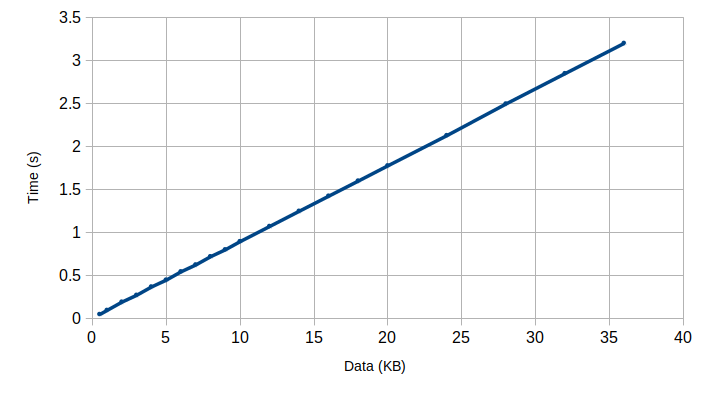
\includegraphics[width=79mm]{Images/comms-time.png}}
	\subfigure[Channel Throughput]{\label{fig:comms:tput}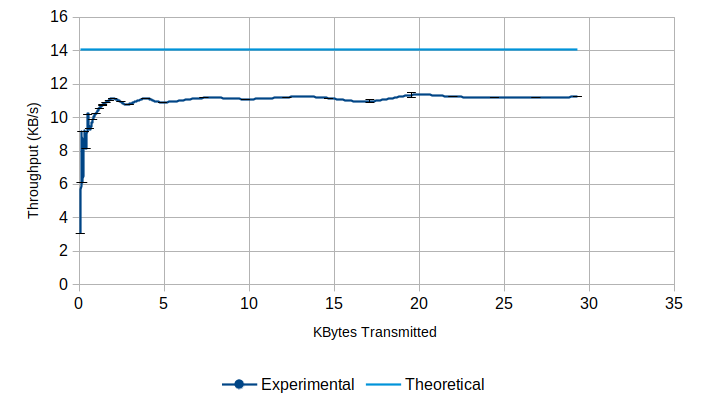
\includegraphics[width=79mm]{Images/comms-tput.png}}
	\caption{Serial port data transmission results}
\end{figure}
The values range from 0.048 seconds for 0.5 KB, to 3.2 s for 36 KB.
In the subsequent graphic, the throughput was calculated from the transmission results.
Figure~\ref{fig:comms:tput} depicts the experimental throughput and theoretical throughput. The theoretical throughput was calculated from the baud rate \(115200/8 = 14.06 KB/s\).
We can observe that the experimental throughput starts at around 10 KB/s for smaller data sizes, and stabilizes around 11 KB/s, as size increases.
We can conclude that the practical throughput is close to the theoretical, and as expected, stabilizes as the data size increases.
The performance of the data channel, in milliseconds, can be modelled by a linear equation \ref{eq:linear-eq}, with values \(T_{total} = 7.281 + 88.638 * KB\), and a median average percentage error of 0.92 \%.

% -----------------------------------------------------
% -----------------------------------------------------
\subsection{SmartFusion2 Services}\label{chap:evaluation:board}

All the security accelerators of the SmartFusion2 SoC were tested. This includes the TRNG, AES accelerator, SHA, HMAC, KeyTree and ECC scalar multiplication and point addition services.
Additionally, a side-channel resistant 128 bit AES core implemented in the FPGA was also tested.
The isolated service processing time and throughput results are presented in Figures \ref{fig:performance:core-time} and \ref{fig:performance:core-tput}. Twenty different data sizes were used in the test, from 0.5 KB up to 36 KB.
\begin{figure}[h!]
	\centering     %%% not \center
	\subfigure[Processing Time]{\label{fig:performance:core-time}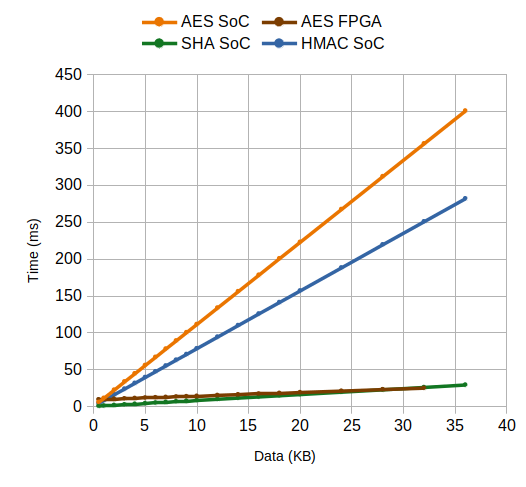
\includegraphics[width=79mm]{Images/core-time.png}}
	\subfigure[Throughput]{\label{fig:performance:core-tput}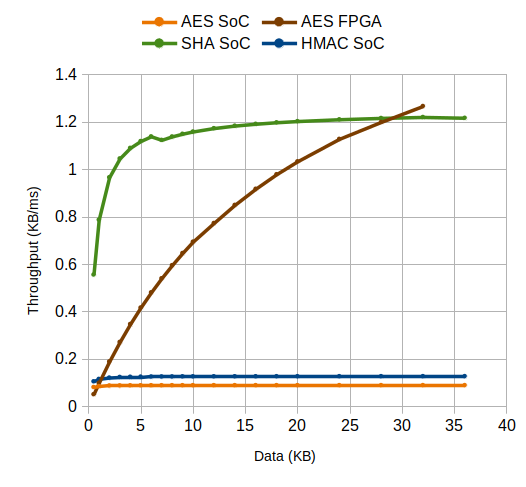
\includegraphics[width=79mm]{Images/core-tput.png}}
	\caption{Security services performance and throughput evolution}
\end{figure}
The AES service was tested with all possible variations. Namely, with 128 bit and 256 bit keys, with all four available modes and with encryption and decryption. Only one result is shown, since there was no variation among them. The AES mode, key size or encryption/decryption operation does not impact the performance. Therefore, there is no performance advantage in choosing CTR mode over CBC mode, or any other mode.
Overall, the AES and HMAC total service time increases faster, compared to SHA, which increases significantly slower.
The ECC services are the slowest, particularly the scalar multiplication (ECDH), with each run taking more than half a second.
The TRNG service was tested by generating 16 random bytes, up to the maximum allowed of 128 bytes. As expected the performance barely increases with the data size.

Figure \ref{fig:performance:core-tput} represents the throughput calculated from the processing time results previously gathered. It shows all services throughput, shown in KB/ms, increases and eventually stabilizes at a specific value. AES stabilizes at around 1.2 KB/ms, and both SHA and HMAC at around 0.1 KB/ms.

All data dependent services followed a near perfect linear evolution, in function of the processed data size, as presented in Table \ref{tab:core-model}.
\begin{table}[h!]
\centering
\def\arraystretch{1.5}
\begin{tabular}{|c|c|c|c|c|c|c|c|}
\hline
Time (ms) & AES    & SHA    & HMAC   & TRNG   & KeyTree & ECC Add. & ECC Mult.	\\ \hline
Constant  & 0.489  & 0.498  & 0.783  & 0.368  & 1.655   & 7.204    & 545.381	\\ \hline
Data (KB) & 11.124 & 0.807  & 7.815  & 0.007  & -       & -	   & -		\\ \hline
MAE       & 0.12\% & 0.84\% & 0.13\% & 2.29\% & -       & -	   & -		\\ \hline
\end{tabular}
\caption{SmartFusion2 services time performance according to a linear model}
\label{tab:core-model}
\end{table}

The error percentages are all below 1\%, except for the TRNG service, proving these models accurately predict the performance of the services.

% -----------------------------------------------------
% -----------------------------------------------------
\subsubsection*{Core/Software Comparison}\label{chap:evaluation:services:software}

The SHA and HMAC performance difference results were enigmatic. The HMAC data dependent portion, 7.815 ms, is nearly 10 times higher than the SHA value, 0.807 ms. This means HMAC's time performance degrades nearly 10 times faster than the SHA performance. This is a surprising result, since the HMAC algorithm is composed of two hash computations and uses SHA-256, so the results are expected to be closer.
The included software implementation of HMAC, SHA and AES were tested for comparison with the SmartFusion2 services. The library used for HMAC and SHA was \cite{ogayHMAC}, and for AES \cite{tinycrypt}. 

\begin{figure}[h!]
	\centering
	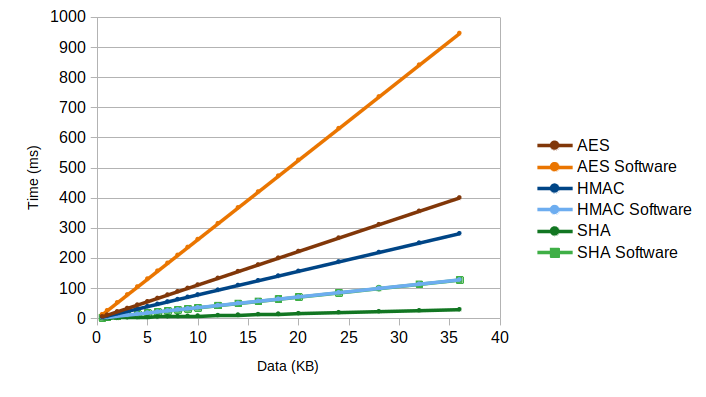
\includegraphics[width=0.7\textwidth]{./Images/software-core-time.png}
	\caption{Performance comparison of the board's cores and a software implementation}
	\label{fig:performance:software-core-time}
\end{figure}

Analyzing the time performance results in Figure \ref{fig:performance:software-core-time}, the SHA and HMAC software results are almost identical, the HMAC is a slightly worse performer. Compared to the software results, the SHA core is significantly faster, and deteriorates very slowly as data size increases. The opposite happens for the HMAC core. It is convincingly a worst performer, compared to both HMAC and SHA software implementations. 
This is an ambiguous result, as there is no clear reason for the HMAC core performance degradation, compared to the SHA core and the software implementations. One could assume it is caused by possible DPA mitigations, but it would still not explain the meaningful discrepancy compared to the SHA core, which also includes these mitigations.
The AES software implementation was tested with encryption in CBC mode and a 256 bit key. As expected, it performs worse than the core service. CTR mode with the same configuration was also tested, and has very similar performance to CBC.

% -----------------------------------------------------
% -----------------------------------------------------
\subsubsection*{Memory Performance}\label{chap:evaluation:services:memory}

The read and write performance of the different device's memories, along with the PUF service were tested. Both eSRAM and eNVM memories were tested from 0.5 KB to 36 KB. The PUF performance was tested from 16 bytes, up to its limit of 512 bytes.
The performance results for the RAM, NVM and PUF are pictured in Figures \ref{fig:performance:memory-time} and \ref{chap:appendixB} of Appendix \ref{chap:appendixB}.

The results show the PUF service barely fluctuates with the data size, since a slot only goes up to 512 bytes. It has an almost constant read and write performance.
Regarding the eNVM, its write performance deteriorates significantly with increasing data sizes.
The RAM write performance is comparable to the eNVM read performance. The RAM read performance was also tested, however, the results are not shown due to its extremely negligible and erratic performance. Instead, a simple increment operation test is presented, in order to show a benchmark for the RAM's performance.

The linear model values were calculated and are presented in Table \ref{tab:memory-model}.
\begin{table}[h!]
\centering
\def\arraystretch{1.5}
\begin{tabular}{|c|c|c|c|c|c|c|}
\hline
Time (ms) & RAM Op. & Write RAM & Read NVM & Write NVM & Fetch PUF & Enroll PUF \\ \hline
Constant  & 0.085     & 0.012     & 0.01     & 8.03      & 128.49    & 747.84  \\ \hline
Data (KB) & 0.34     & 0.014     & 0.02     & 298.10    & 0.006     & 0.008  \\ \hline
MAE       & 1.90\%    & 2.76\%    & 3.76\%   & 0.31\%    & 0.17\%    & 0.06\%  \\ \hline
\end{tabular}
\caption{Smartfusion2 memory performance time values according to a linear model}
\label{tab:core-model}
\end{table}



% -----------------------------------------------------
% -----------------------------------------------------
\subsection{Implemented Services}\label{chap:evaluation:services}

This section presents the performance results of the implemented services from Chapter \ref{chap:implementation}. Each service's performance depends on the used accelerator's, memory access and implemented logic.
The tested services were, encryption and authentication, decryption and authentication, both using the AES accelerator and the HMAC software implementation; the key import service, using the AES, HMAC and PUF cores, ECDSA and ECDH, both using the ECC scalar multiplication accelerator. ECDSA also uses the ECC point addition core. It is worth noting that the encryption service also uses the TRNG service, to generate a random IV. 
The continuous encryption and decryption services used a 36 KB buffer for data.

The performance of the key import service is depicted in Figure \ref{fig:performance:nvm-puf-time} in Appendix \ref{chap:appendixB}. The figure compares this service to the PUF read and write performance, in order to compare both key storage options.
Just as the PUF service, the key import service barely varied, due to the small data interval.
Analyzing the results in Figure	\ref{fig:performance:services-time} of Appendix	\ref{appendixB}, both encryption/decryption and authentication services have very similar values, due to being based on the same service's and AES encryption and decryption having no discernible performance difference.

\begin{figure}[h!]
	\centering
	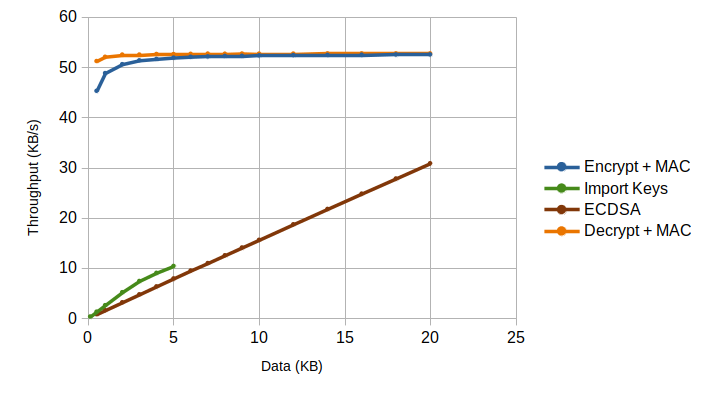
\includegraphics[width=0.7\textwidth]{./Images/services-tput.png}
	\caption{Continuous encryption and decryption throughput evolution for increasing input data sizes}
	\label{fig:performance:services-tput}
\end{figure}
Figure \ref{fig:performance:services-tput} plots the throughput (KB/s) values for the continuous encryption and decryption services. Throughput steadily increases and stabilizes after 10 KB, at around 68 KB/s, for both services.

Similarly to the previous tests, the time performance results evolve linearly. The obtained values are presented in Table \ref{tab:services-model}.
\begin{table}[h!]
\centering
\def\arraystretch{1.5}
\begin{tabular}{|c|c|c|c|c|c|c|}
\hline
	Time (ms) & Encrypt Data  & Decrypt Data  & Import Keys & ECDSA & ECDH   \\ \hline
	constant  & 2.1    & 0.847  & 368.994  & 629.932 & 964.535 \\ \hline
	data      & 14.678 & 14.681 & 18.518 & 0.937 & - \\ \hline
	MAE	  & 0.10\% & 0.12\%  & 2.86\% & 0.18\% & - \\ \hline
\end{tabular}
\caption{Implemented services time values according to a linear model}
\label{tab:services-model}
\end{table}

% \begin{table}[]
% \centering
% \def\arraystretch{1.5}
% \begin{tabular}{|c|c|c|c|c|c|c|}
% \hline
% Time/Service   & Encrypt + MAC	  & Decrypt + MAC  & Import Keys & ECDSA   \\ \hline
%         constant (ms) & 29.413 & 29.413 & 0.002 & 0.138 \\ \hline
%         data (ms) & 6.704 & 6.704 & 1.942 & 1.542 \\ \hline
%         MAE \%	   & 1.032 & 1.006 & 0.127 & 1.760 \\ \hline
% \end{tabular}
% \caption{Implemented services throughput model values}
% \label{tab:services-model}
% \end{table}


By analysing the calculated models we can detect a difference in the constant component of the encryption service compared to decryption. This is due to the random IV generation with the board's TRNG on the encryption service.
Key generation with ECDH performs at a constant time of 578.092 ms, and ECDSA at 629.434 ms.
Scalar multiplication has a big impact on the performance for both ECDH and ECDSA.
The median average percentage error for the continuous encryption/decryption models is below 0.19\%, so the models almost perfectly represent its performance.% The import keys service model has the highest error with 2.86\%.

% ---------
As mentioned previously, the continuous encryption/decryption with MAC implementation uses a 36 KB buffer. Thus, the service can receive chunks of up to 36 KB at a time.
Since the server is continuous and can encrypt and authenticate a limitless amount of data, the buffer does not necessarily need to be the maximum possible value. The service might have comparable performance with a smaller buffer, which frees up memory space for further implementation code.

In order to understand the impact of the buffer size on performance, the previous test on the encryption and MAC services was repeated, with varying buffer sizes, from 0.1 KB up to 35 KB.
All tests revealed the same linear performance behaviour as the previous test with a 36 KB buffer. In order to compare and understand the service performance for each buffer buffer size, the maximum, minimum and average throughput are pictured in Figure \ref{fig:performance:buffer-tput}.
\begin{figure}[h!]
	\centering
	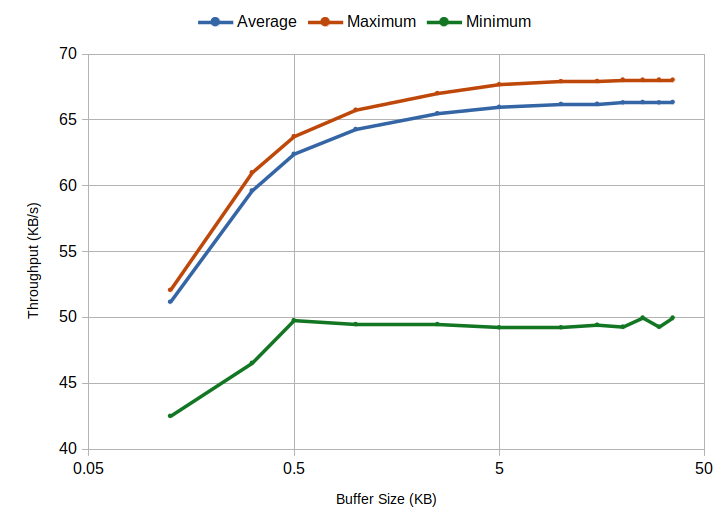
\includegraphics[width=0.7\textwidth]{./Images/buffer-tput.png}
	\caption{Continuous encryption and MAC throughput evolution with increasing buffer sizes}
	\label{fig:performance:buffer-tput}
\end{figure}
The worst performance, and therefore lower throughput, is achieved with the lowest data size of 0.5 KB. The throughput eventually stabilizes around its maximum value, with data sizes higher than 20 KB.
A smaller range from the minimum to maximum throughput, for a particular buffer size, indicates the throughput increases slower, as data size increases.

Analysing the plot, the average throughput significantly increases from 0,1 KB up until 5 KB, after which, the average throughput stabilizes around 66 KB/s and the maximum at 68 KB/s. 
If the goal is to maximize throughput, there is no advantage in using a buffer bigger than 10 KB. Even a 5 KB buffer has almost identical performance. 

The minimum throughput spikes at 49.5 KB/s with a 0.5 KB buffer, then is relatively constant. As discussed before, the minimum throughput is achieved at the lowest processed data size of 0.5 KB. Thus, by analysing the graphic, the minimum throughput increases until the buffer size (0.5 KB) is equal to the amount of data being processed (0.5 KB). After that, there is no benefit in having a bigger buffer size, since the lowest amount of processed data is still 0.5 KB.
Therefore, if the amount of data which will be processed is known beforehand, the system can be configured with a buffer of equal size, so as to maximize throughput.
% For higher data sizes, where the maximum throughput is achieved, a buffer size of at least 5 KB is a good choice. However, if the system mainly receives small data of around 0.5 KB, the minimum throughput becomes relevant. It becomes stable from a buffer of 0.5 KB, up to a 35 KB. For this use case, if memory space is needed, a 0.5 KB buffer is acceptable. The extra saved memory can be used to implement more functionalities.

% -----------------------------------------------------
% -----------------------------------------------------
\section{Requirements}\label{chap:evaluation:requirements}

This section evaluates the fulfilled requirements of the developed system, defined in Chapter \ref{chap:problem:requirements}.
The SmartFusion2 SoC is a portable board, with a robust set of security services.
Compared to the existing HSMs on the market, this device is one of the cheapest, so it is adequate for distribution among several users. Market HSMs go from 650€ up to \$39,000 \cite{HSMpriceArticles}, \cite{HSMPresentationPrices}. A M2S090TS SmartFusion2 evaluation kit is priced at 384 € \cite{smartfusionPrice}.

The board provides encryption and authentication with AES and HMAC, a secure storage service for keys, and shared key generation with ECDH. It provides tamper detection capabilities, secure boot and zeroization.
It has the necessary functionalities to provide authentication and confidentiality to communications, which is the main requirement of the system.
The developed prototype uses the board's services, except for the HMAC software implementation, and all keys are stored securely.

The developed key management solution allows the periodic replacement of keys. Therefore, communications with new entities, with similar devices, can be established.
Users must authenticate themselves to the device, using its authentication PIN. This way entities can manage which users have access to the device, on behalf of the entity.
Whenever a tamper attempt or error is detected, the device does not accept any more API calls, and can be completely erased. This mitigates potential physical attacks and data leaks.
A PKCS\#11 API was developed to expose the device's functionalities and increase device interoperability.

% -----------------------------------------------------
% -----------------------------------------------------
\section*{Summary}\label{chap:evaluation:summary}

In this chapter, the implemented system performance was thoroughly tested. Starting with the communication channel performance, then the SmartFusion2 security accelerators and implemented services. In order to accurately predict the performance of the studied services, performance models were calculated from the performance results. These models allow anyone using this device to accurately study and predict the performance of services, implemented on the board. Thus, this chapter provides a robust study of the SmartFusion2 board, its services characteristics, performance, as well as possible services to implement, feature trade offs and efficiency concerns.
